
\baituluan{toiuu201701:b01}{
(3 điểm)
Một nhà đầu tư có 2 tỉ đồng, muốn đầu tư vào 4 lĩnh vực: chứng khoán. công trái, gửi tiết kiệm và bất động sản. Biết lãi suất hàng năm của các lĩnh vực đầu tư như sau:
\begin{center}
\renewcommand{\arraystretch}{1.25}
\begin{tabular}{| l | c |}
\hline
Lĩnh vực đầu tư&Lãi suất hàng năm\\ 
\hline
Chứng khoán&20\%\\ 
Công trái&12\%\\ 
Gửi tiết kiệm&10\%\\ 
Bất động sản&15\%\\
\hline 
\end{tabular}
\end{center}

Ngoài ra để giảm thiểu mức rủi ro, nhà đầu tư cho rằng không nên đầu tư vào chứng khoán vượt quá 40\% tổng vốn đầu tư, còn đầu tư vào công trái và gửi tiết kiệm phải ít nhất là 25\% tổng vốn đầu tư và tiền gửi tiết kiệm phải ít nhất là 100 triệu đồng.\\
 Hãy lập mô hình toán học kế hoạch phân bổ vốn đầu tư sao cho tổng thu nhập hàng năm là lớn nhất.
% b) Chuyển mô hình bài toán về bài toán đối ngẫu.
}{
Gọi $x_1, x_2, x_3, x_4$ tương ứng là số tiền triệu đồng đầu tư vào chứng khoán, công trái, gửi tiết kiệm, bất động sản.\\
Cực đại tổng thu nhập hàng năm:
$$ f=0,2x_1+0,12 x_2+0,1 x_3 + 0,15 x_4 \mbox{ (triệu đồng)}\rightarrow \max$$
Các ràng buộc:\\
Tổng số tiền đầu tư không vượt quá số tiền hiện có
$$x_1+x_2+x_3+x_4\le 2000 \mbox{ (triệu đồng)}$$
Đầu tư vào chứng khoán với điều kiện
$$x_1\le 0,4(x_1+x_2+x_3+x_4)$$
Đầu tư vào công trái và gửi tiết kiệm
$$x_2+x_3\ge 0,25(x_1+x_2+x_3+x_4)$$
Điều kiện gửi tiết kiệm tối thiểu: $x_3\ge 100.$
Điều kiện không âm $x_j\ge 0, j=1, 2, 3, 4.$

Mô hình của bài toán là: Tìm $(x_1, x_2, x_3, x_4)$ sao cho
$$ f=0,2x_1+0,12 x_2+0,1 x_3 + 0,15 x_4 \rightarrow \max$$
Với hệ ràng buộc
\begin{equation*}
\left\{
\begin{array}{r r r r l }
x_1&+x_2&+x_3&+x_4&\le 2000 \\ 
-0,6x_1&+0,4x_2&+0,4x_3&+0,4x_4&\ge 0 \\ 
-0,25x_1&+0,75x_2&+0,75x_3&-0,25x_4&\ge 0 \\ 
x_3&\ge 100 \\ 
\multicolumn{4}{l}{x_j\ge 0,\quad j = 1, 2, 3,4.}\\
\end{array}
\right.
\end{equation*}
}

\baituluan{toiuu201701:b02}{%1\\
(3 điểm)  Giải bài toán quy hoặc tuyến tính sau bằng hình học:
$$L(x,y)=20x+40y\rightarrow\max$$
$$\begin{cases}
\systeme{
6x+y\ge 18,:
x+4y\ge 12,:
2x+y\ge 10,}\\
x,y\ge 0.
\end{cases} $$
}{
Giải bằng phương pháp hình học. Miền các phương án được xác định bằng đa giác lồi mở
$xABCDy$ với $A(12,0), B(4,2), C(2,6), D(0,18)$. Biểu diễn vectơ pháp tuyến $\vec{n}=(1,2)$ và hàm mục tiêu $L(x,y)=20x+40y$ như hình vẽ.

\begin{figure}[!htp]
\centering
%\input hinh24.tex
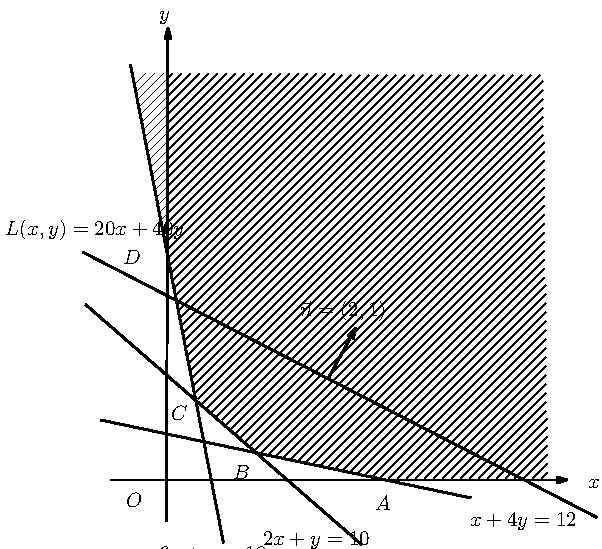
\includegraphics[scale =0.7]{hinh24}
\caption{}\label{fig:2}
\end{figure}

Di chuyển đường hàm mục tiêu ngược với $\vec{n}$ tới vô cùng. Vậy bài toán không có phương án tối ưu.
}

\baituluan{toiuu201701:b03}{%3
(4 điểm)
Xét bài toán quy hoạch tuyến tính sau đây
$$ f=5x_1+4x_2+6x_3\rightarrow \min$$
\begin{equation*}
\left\{
\begin{array}{r r r l }
2x_1&+4x_2&+3x_3&\ge 48 \\ 
3x_1&+2x_2&+3x_3&\ge 30 \\ 
x_1&+3x_2&+4x_3&\ge 23 \\ 
\multicolumn{4}{l}{x_j\ge 0,\quad j = 1, 2, 3.}\\
\end{array}
\right.
\end{equation*}

a) Hãy đưa bài toán về dạng chính tắc.

b) Giải bài toán bằng phương pháp đơn hình.
}{
a) Đưa bài toán về dạng chính tắc
$$ f=5x_1+4x_2+6x_3\rightarrow \min$$
\begin{equation*}
\left\{
\begin{array}{r r r r r  r l }
2x_1&+4x_2&+3x_3&-x_4&&&= 48 \\ 
3x_1&+2x_2&+3x_3&&-x_5&&= 30 \\ 
x_1&+3x_2&+4x_3&&&-x_6&= 23 \\ 
\multicolumn{6}{l}{x_j\ge 0,\quad j = 1, 2, 3, 4, 5, 6.}\\
\end{array}
\right.
\end{equation*}
b) Ta biến đổi để xuất hiện biến cơ bản như sau:  Giữ nguyên phương trình thứ nhất, đem nó trừ đi lần lượt các phương trình thứ 2 và 3 cho kết quả mới. Ta có bài toán tương đương
$$ f=5x_1+4x_2+6x_3\rightarrow \min$$
\begin{equation*}
\left\{
\begin{array}{r r r r r  r l }
2x_1&+4x_2&+3x_3&-x_4&&&= 48 \\ 
-x_1&+2x_2&&-x_4&+x_5&&= 18 \\ 
x_1&+x_2&-x_3&-x_4&&+x_6&= 25 \\ 
\multicolumn{6}{l}{x_j\ge 0,\quad j = 1, 2, 3, 4, 5, 6.}\\
\end{array}
\right.
\end{equation*}
Ta đưa về bài toán mở rộng
$$ f=5x_1+4x_2+6x_3\qquad +Mx_7\rightarrow \min$$
\begin{equation*}
\left\{
\begin{array}{r r r r r  r r l }
2x_1&+4x_2&+3x_3&-x_4&&&+x_7&= 48 \\ 
-x_1&+2x_2&&-x_4&+x_5&&&= 18 \\ 
x_1&+x_2&-x_3&-x_4&&+x_6&&= 25 \\ 
\multicolumn{6}{l}{x_j\ge 0,\quad j = 1, 2, 3, 4, 5, 6,7.}\\
\end{array}
\right.
\end{equation*}
Trong đó $x_7$ là biến giả, $M>0$ rất lớn.
\begin{center}
\begin{longtable}{| l | l | l | l  l  l  l  l  l  l |}
\hline
$x_B$&$c_B$&PA&$x_1$&$x_2$&$x_3$&$x_4$&$x_5$&$x_6$&$x_7$\\ 
&&&5&4&6&0&0&0&M\\ 
\hline
$x_7$&M&48&[2]&4&3&-1&0&0&1\\ 
$x_5$&0&18&-1&2&0&-1&1&0&0\\ 
$x_6$&0&25&1&1&-1&-1&0&1&0\\
\hline 
f &M&48&2&4&3&-1&0&0&0\\ 
\cline{2-10}
&&0&-5&-4&-6&0&0&0&0\\ 
\hline
$x_1$&5&24&1&2&3/2&-1/2&0&0&\\ 
$x_5$&0&42&0&[4]&3/2&-3/2&1&0&\\ 
$x_6$&0&1&0&-1&-5/2&-1/2&0&1&\\ 
\hline
f&&120&0&6&3/2&-5/2&0&0&\\ 
\hline
$x_1$&5&3&1&0&3/4&1/4&-1/2&0&\\ 
$x_2$&4&21/2&0&1&3/8&-3/8&1/4&0&\\ 
$x_6$&0&23/2&0&0&-17/8&-7/8&1/4&1&\\ 
\hline
f&&57&0&0&-3/4&-1/4&-3/2&0&\\ 
\hline
\end{longtable}
\end{center}
Bài toán đã cho có phương án tối ưu duy nhất là
$x^*=(3, 21/2, 0)$ và $f_{\min}=57$.
}
%%%%%%%%%%%%%%%%%%%%%%%%%%%%%%%%%%%%%%%%%%%%%%%
% \baituluan{toiuu201701:b01}%3
% Cho số liệu bài toán vận tải và ma trận $(c_{ij})$ như sau:
% 
% $(a_i)=(100, 80, 20)^t$ \qquad $(b_j)=(60, 70, 40, 30)$
% 
% $(c_{ij})=\begin{bmatrix}
% 2&1&4&3\\ 
% 5&3&2&6\\ 
% 6&2&1&5\\ 
% \end{bmatrix}$ 
% 
% a) Viết lại nội dung bài toán vận tải trên như bài toán quy hoạch tuyến tính.
% 
% b) Lập bảng vận tải cho bài toán trên.
% 
% c) Tìm phương án xuất phát theo phương pháp cực tiểu cước phí.
% 
% d) Giải bài toán vận tải trên theo phương pháp quy 0 cước phí các ô chọn.
% }{
% a) b) c) như trong sách.
% 
% d) Kết quả nghiệm
% 
% $x^*=\begin{bmatrix}
% 60&10&0&30\\ 
% 0&60&20&0\\ 
% 0&0&20&0\\ 
% \end{bmatrix}$ 
% ,\quad $f(x^*)=460.$
% \end{traloi}
% \end{cauhoi}
% 
% \vspace*{1cm}
% {\bf Chú ý:} Sinh viên không được mang sách giáo trình và vở ghi chép vào phòng thi.
% \Closesolutionfile{goiytraloi}
% \newpage
% \Readsolutionfile{goiytraloi}

% \end{document}


